%!TEX root = nonabelions.tex

\chapter{Topological Quantum Computation}\label{chap:tqc}

This chapter can be seen as an application of non-abelian anyons to perform topological quantum computation. For further details see \cite{nayak,freedman kitaev larsen wang,shor fault-tolerant,braid topologies,ainsworth slingerland}.

The motivation for considering topological quantum computers is that most existing attempts at constructing quantum computers, such as ion traps, superconducting Josephson junctions and optical lattices, all share one pressing limitation; decoherence. Quantum decoherence is the effect where a quantum system, such as one implementing a quantum computer, essentially looses information to the environment. When a system is coupled to the environment, the dynamics of the system is no longer necessarily unitary, however, the total system still evolves unitarily, but it is not feasible to keep track of the exact state of the environment. The environment can introduce noise simply from heat, this eventually leads to errors in the quantum information. Efforts of completely isolating quantum systems from the environment have yet not proved successful. In some cases this can be (partially) remedied by quantum error correction algorithms.

Topological quantum computation solves the issue of decoherence by representing the quantum information in a topological state, namely the braids that we have discussed in length in previous chapters. A braid is topological in the sense that homotopy equivalent braid represent the same physical state, characterized solely by the braid group representation. There may still be an error rate, however, it decreases exponentially with the spatial separation the computational anyons \cite{freedman kitaev larsen wang}, and is thus not an issue in principle.

Abelian anyons cannot be used for quantum computation, since the fusion space of abelian anyons is necessarily one-dimensional while a qubit is two-dimensional. In \cref{sec:computing with fibonacci} we shall see how Fibonacci anyons, as introduced in \cref{fibonacci anyons}, can be used to perform quantum computation. First we give an introduction to quantum computation in general, defining the concepts that are built upon in topological quantum computation.


\section{Introduction to quantum computation}\label{sec:intro qc}

% Skipped topics: Mixed states, quantum vs classical complexity, quantum informatics

This section gives a concise introduction to quantum computation, this discussion is self-contained and can be read in isolation from the rest of the thesis, or skipped if the reader is already familiar with the concepts. The mentioned results and further information can be found in \cite{nielsen chuang}.



\subsection{Qubits}

Quantum computation performs computation by manipulating qubits, similar to how classical computation performs computation by manipulating bits. A classical bit consists of exactly two discrete states, $0$ and $1$. A qubit is much richer, it has two orthonormal states, $\ket{0}$ and $\ket{1}$, analogous to the classical case, in addition to this a qubit can also be in linear combinations (superpositions) of these states. In other words, a qubit is a two-dimensional quantum state
\begin{equation}
  \ket{\psi} = a e^{i\alpha} \ket{0} + b e^{i\beta} \ket{1}.
\end{equation}
As it stands, $\ket{\psi}$ depends on four real parameters, $a\ge 0$, $b\ge 0$, $\alpha$ and $\beta$. However, $a^2$ and $b^2$ are the probabilities of finding the state $\ket{\psi}$ in state $\ket{0}$ and $\ket{1}$, respectively, the superposition cannot be directly observed. This is the Born rule. Because of this, we must have $a^2+b^2 = 1$, thus fixing one parameter $a = \sqrt{1-b^2}$ which ranges between $0$ and $1$. Furthermore, the global phase of a quantum system is not physical, see \cref{sec:global vs relative phase}, thus an overall factor $e^{i\omega}$ is not visible and we have
\begin{equation}
  \ket{\psi} = e^{i\omega}\left( a e^{i(\alpha-\omega)} \ket{0} + b e^{i(\beta-\omega)} \ket{1} \right)
\end{equation}
where $\omega$ is not known. Therefore, information of both $\alpha$ and $\beta$ is not available, only the difference $\beta-\alpha$, as seen by eliminating $\omega$ by letting $\omega = \alpha$ so that we have
\begin{equation}
  \ket{\psi} = e^{i\omega}\left( a\ket{0}+be^{i(\beta-\alpha)}\ket{1} \right),
\end{equation}
or if we instead choose $\omega = \beta$ we put the relative phase $\alpha-\beta$ on the $\ket{0}$ state
\begin{equation}
  \ket{\psi} = e^{i\omega}\left( ae^{i(\alpha-\beta)}\ket{0}+b\ket{1} \right).
\end{equation}
In conclusion, the state $\ket{\psi}$ is determined by two real parameters, $0 \le a \le 1$, and $\beta - \alpha$ which is $2\pi$ periodic. Finally, note that for $a = 0$ and $a = 1$, the relative phase is no longer physical, it is part of the global phase. In conclusion, the elements of the Hilbert space are not in one-to-one correspondence with physical states. We now characterize the space obtained by identifying physically indistinguishable states.



\subsection{The Bloch sphere}

The space of the two parameters determining a qubit is the Cartesian product of the interval $[0,1]$ representing the possible values for $a$, and the circle $[0,2\pi]$ with endpoints $0$ and $2\pi$ identified, representing the possible values for the relative phase $\beta - \alpha$. Thus, we have a cylinder with the property that all points on the circles at $a = 0$ and $a = 1$, respectively, are identified, since the relative phase is non-physical at these points. The resulting space of physically distinguishable states is topologically equivalent to a sphere. This space is called the Bloch sphere, see \cref{fig:bloch sphere}. The Bloch sphere can be parameterized by spherical coordinates and every qubit state can be written uniquely as
\begin{equation}
  \ket{\psi} = \cos(\theta/2) \ket{0} + e^{i\phi}\sin(\theta/2) \ket{1}
\end{equation}
where $0 \le \theta \le \pi$ and $0 \le \phi < 2\pi$. This provides geometric intuition for single-qubit operations.

\begin{figure}[!htb]
  \centering
  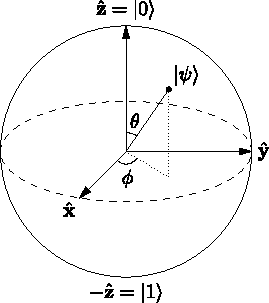
\includegraphics{img/bloch-sphere.pdf}
  \caption{The Bloch sphere, uniquely representing all states of a qubit.}
  \label{fig:bloch sphere}
\end{figure}



\subsection{Multi-qubit systems}

We can define $d$-dimensional analogues of qubits, referred to as qudits, by
\begin{equation}
  \ket{\psi} = a_0 e^{i\theta_0} \ket{0} + \ldots + a_{d-1} e^{i \theta_{d-1}} \ket{d-1}.
\end{equation}
Similarly, classical bits can be generalized to computational units of $d$ states. However, the most common approach to have a larger computational space is to instead introduce additional qubits. The state space of a single qubit is Hilbert space $\mathbb{C}^2$, the state space of $n$ qubits is the Hilbert space $ℋ_n \cong (\mathbb{C}^2)^{\otimes n} \cong \mathbb{C}^{2n}$ and the basis states are
\begin{equation}
  |000⋯0⟩, |100⋯0⟩, |010⋯0⟩, |110⋯0⟩, |001⋯0⟩, …, |11⋯1⟩,
\end{equation}
where we use the notation
\begin{equation}
  \ket{x_1x_2\cdots x_n} = \ket{x_1}\otimes\ket{x_2}\otimes\cdots\otimes\ket{x_n}.
\end{equation}

Note the striking difference between quantum and classical bits:
The state of one classical bit is determined by one number ($0$ or $1$).
The state of one qubit is determined by two continuous parameters, the amplitude trade-off and the relative phase.
The state of $n$ classical bits is determined by $n$ numbers (each $0$ or $1$), the number of parameters grows linearly.
The state of $n$ qubits is determined by $2^{n+1}-2$ continuous parameters, the term $-2$ is due to the fact that two parameters are fixed by normalization and the global phase. These parameters are the coefficients in the linear combination of basis states, the number of parameters grows exponentially. In conclusion, $n$ qubits can be seen as holding exponentially more information than classical bits. However, only $n$ classical bits can be read out from $n$ qubits, because a measurement collapses entanglement. This is an important consideration when designing quantum algorithms.

Quantum information can be entangled across qubits. As an example, consider the case of $n = 2$ qubits, the state
\begin{equation}
  \frac{1}{√2}\big(|0⟩⊗|1⟩ + |1⟩⊗|0⟩\big)
\end{equation}
is entangled, the two qubits are necessarily in opposite states. If one knows that the first qubit is in state $|0⟩$ then the second qubit is necessarily in state $|1⟩$, and vice versa. Both possibilities occur with probability $1/2$. The notion of entanglement is captured exactly by the following definition.

\begin{definition}
  A state $|ψ⟩ ∈ ℋ = ⨂ⱼHⱼ$ is said to be entangled if it cannot be written on the form $⨂ⱼ|ψⱼ⟩$.
\end{definition}


\subsection{Computing with qubits}

Now, how do we actually compute with qubits? The dynamics of every quantum system is determined by the Schrödinger equation,
\begin{equation}
  i\frac{∂}{∂t}\ket{\psi(t)} = H\ket{ψ(t)}
\end{equation}
for some Hamiltonian $H$, necessarily being Hermitian and $\ket{\psi(t)}$ an element of a complex Hilbert space. The solution to this equation is
\begin{equation}
  \ket{\psi(t)} = e^{-iHt}\ket{\psi(0)}.
\end{equation}
Since every unitary matrix can be written on the form $e^{-iHt}$, we see that quantum states have unitary time evolution. Quantum computation is performed by taking an initial state $\ket{\psi}$, often $\ket{\psi} = \ket{00\cdots0}$, and unitarily evolving it by acting with a unitary operator $U$ on $\ket{\psi}$ to give a new state $U\ket{\psi}$. If the system consists of $n$ qubits, the unitary operator is an element of $U(2)^{\otimes n} = U(2^n)$, where $U(m)$ is the group of $m$-dimensional unitary matrices. Similarly, evolution of qudits is described by $U(d)$ matrices. Such a unitary action is achieved by appropriately manipulating the Hamiltonian $H$. How this happens in practice depends heavily on how the qubit system is implemented. In the case of ion traps, single qubit gates are performed by shooting a lase at the ion, and entanglement is established via electromagnetic coupling. In the case of non-abelian anyons, quantum gates are implemented via braids, as we shall see in \cref{sec:computing with fibonacci}. Note that since unitary operators are invertible, quantum computation is necessarily reversible (provided that no wave function collapse occurs).



\subsection{Quantum gates and universality}\label{sec:gates and universality}

Quantum gates refer to a finite set of specific unitary operators, ones that are implemented in the given physical system. Other unitary operations can then be implemented in terms of the basic quantum gates, expressed as a finite product of quantum gates. Ideally, the set of quantum gates can implement any unitary operator, if this is the case the set of quantum gates is called universal. To be precise, this is never possible since the set of unitary operators is uncountable while finite sequences of finite sets (representing products of quantum gates) is countable. Instead, universality of a set of quantum gates requires that any unitary operator can be approximated to arbitrary precision with a finite sequence of quantum gates. That is, the subset of operators generated by the set of gates is dense in $U(d)$.

Unitary operators can be interpreted as rotations in Hilbert space, single-qubit operations are effectively rotations on the Bloch sphere.

When performing explicit calculations, one often represents the basis states as the vectors
\begin{equation}
  \ket{0} = \begin{pmatrix} 1 \\ 0\end{pmatrix}, \quad \ket{1} = \begin{pmatrix} 0 \\ 1 \end{pmatrix}
\end{equation}
and the tensor product (for multi-qubit systems) is computed as the Kronecker product
\begin{equation}
  \begin{pmatrix} a \\ b \end{pmatrix} \otimes \begin{pmatrix} c \\ d \end{pmatrix}
  = \begin{pmatrix} ac \\ ad \\ bc \\ bd \end{pmatrix}.
\end{equation}
This can be repeated for any number of tensor products. Thus, we represent quantum gates as matrices. Common single-qubit gates include the Pauli operators
\begin{equation}
  σₓ  = σ₁ = \begin{pmatrix} 0 & 1 \\ 1 & 0 \end{pmatrix}, \quad
  σ_y = σ₂ = \begin{pmatrix} 0 & -i \\ i & 0 \end{pmatrix}, \quad
  σ_z = σ₃ = \begin{pmatrix} 1 & 0 \\ 0 & -1 \end{pmatrix}
\end{equation}
rotating the state $\pi$ radians along the $x$-, $y$- and $z$-axis, respectively. Note that $\sigma_x$ corresponds to the classical NOT gate, flipping $\ket{0}$ and $\ket{1}$. Often one writes $σ₀ = I$. The Pauli matrices are especially interesting since the set $\{σ₀,σ₁,σ₂,σ₃\}$ is a basis for $GL₂(ℂ)$. Furthermore, $c₀σ₀ + c₁σ₁ + c₂σ₂ + c₃σ₃$ is Hermitian precisely when the coefficients $c₀,…,c₃$ are real. This is verified by straight-forward calculations.

The phase shift gate
\begin{equation}
  R(\phi) =
  \begin{pmatrix}
    1 & 0 \\
    0 & e^{i\phi}
  \end{pmatrix};\quad
  \ket{0} \mapsto \ket{0},\quad
  \ket{1} \mapsto e^{i\phi} \ket{1}
\end{equation}
generalizes $σ_z$, since $R(\pi) = \sigma_z$.

None of these gates introduce superpositions, for this one can use the Hadamard gate
\begin{equation}\label{eq:hadamard}
  H = \frac{1}{\sqrt{2}} \begin{pmatrix} 1 & 1 \\ 1 & -1 \end{pmatrix}
\end{equation}
which maps the basis states according to
\begin{equation}
  \ket{0} \mapsto \frac{1}{\sqrt{2}} \left( \ket{0} + \ket{1} \right), \quad
  \ket{1} \mapsto \frac{1}{\sqrt{2}} \left( \ket{0} - \ket{1} \right).
\end{equation}
This gate has no classical counterpart.

Single-qubit cannot introduce entanglement, which is inherently a property of multiple qubit. For this, one can use the CNOT gate
\begin{equation}
  \operatorname{CNOT} =
  \begin{pmatrix}
    1 & 0 & 0 & 0 \\
    0 & 1 & 0 & 0 \\
    0 & 0 & 0 & 1 \\
    0 & 0 & 1 & 0
  \end{pmatrix} : \mathbb{C}^2 ⊗ \mathbb{C}^2 \to \mathbb{C}^2 ⊗ \mathbb{C}^2
\end{equation}
that acts on pairs of qubits, flipping the second qubit if and only if the first qubit is in the state $\ket{1}$, i.e.
\begin{equation}
  \begin{aligned}
    \ket{00} \mapsto \ket{00},\quad &\quad \ket{10} \mapsto \ket{11}. \\
    \ket{01} \mapsto \ket{01},\quad &\quad \ket{11} \mapsto \ket{10}.
  \end{aligned}
\end{equation}
It is called a controlled-NOT gate, similarly one defines the controlled-$U$ gate for any single-qubit gate $U$. A fundamental result of quantum computing shows that the set $\{H, \operatorname{CNOT}, R(\pi/4)\}$ is universal \cite{nielsen chuang}. In order have a single universal gate, it must act on at least three qubits, an example of this is the Deutsch gate $D(\theta)$ give by
\begin{equation}
  D(\theta) = \ket{a,b,c} \mapsto
  \begin{cases}
    i \cos(\theta) \ket{a,b,c} + \sin(\theta) \ket{a,b,1-c} & \mbox{for }a=b=1 \\
    \ket{a,b,c} & \mbox{otherwise,}
  \end{cases}
\end{equation}
or represented as a matrix
\begin{equation}
  D(\theta) =
  \begin{pmatrix}
    1 & 0 & 0 & 0 & 0 & 0 & 0 & 0 \\
    0 & 1 & 0 & 0 & 0 & 0 & 0 & 0 \\
    0 & 0 & 1 & 0 & 0 & 0 & 0 & 0 \\
    0 & 0 & 0 & 1 & 0 & 0 & 0 & 0 \\
    0 & 0 & 0 & 0 & 1 & 0 & 0 & 0 \\
    0 & 0 & 0 & 0 & 0 & 1 & 0 & 0 \\
    0 & 0 & 0 & 0 & 0 & 0 & i\cos(\theta) & \sin(\theta) \\
    0 & 0 & 0 & 0 & 0 & 0 & \sin(\theta) & i\cos(\theta)
  \end{pmatrix}.
\end{equation}
This can be seen as a controlled-controlled-$\begin{pmatrix}i\cos(\theta)&\sin(\theta)\\\sin(\theta)&i\cos(\theta)\end{pmatrix}$ gate. It is in general a purely quantum gate, as it introduces phase shift, superposition and entanglement. In classical computing, a three bit gate known as the Toffoli gate is universal, it is precisely the $D(\pi/2)$ gate, i.e.\ the CCNOT (Controlled CNOT) gate. This shows that any classical computation can be performed as a quantum computation. In fact, the other direction also holds, classical computation can simulate quantum computation. However, in general this requires an exponential increase in the number of bits.

\subsection{Quantum algorithms}

One of the most well-known quantum algorithms is Shor's algorithm for integer factorization. It runs exponentially faster than the fastest known classical factoring algorithm. Time complexity is essentially determined by the number of gates needed to perform the algorithm. It is worth noting that quantum and classical gates are physically very different. Many quantum algorithms, including Shor's, gain their exponential speedup from using the quantum Fourier transform (QFT). Because of this, the QFT will serve as a good example of how quantum algorithms work. We now describe the QFT in some detail.

Define the $n$-qubit QFT on the basis states as
\begin{equation}
  \mathcal{F}\ket{k} = \frac{1}{\sqrt{2^n}} \sum_{j=0}^{2^n-1} e^{2πijk/2^n} \ket{j}
\end{equation}
where we use the notation $\ket{k_1k_2\cdots k_n} = \ket{k}$ where $k$ is the decimal representation of the binary string $k_1k_2\cdots k_n$.
That is, the QFT transforms the amplitudes of a general state according to
\begin{equation}
  \mathcal{F} \left( \sum_{k=0}^{2^n-1} x_k \ket{k} \right) = \sum_{k=0}^{2^n-1} y_k \ket{k}
\end{equation}
where
\begin{equation}
  y_{k} = \frac{1}{\sqrt{2^n}} \sum_{j=0}^{2^n-1} x_j e^{2\pi i j k / 2^n}.
\end{equation}
It is straight-forward to show that this transformation indeed is unitary.
The vector $(y_k)_{k=0}^{2^n-1}$ is precisely the classical discrete Fourier transform (DFT) of the vector $(x_k)_{k=0}^{2^n-1}$. Thus, QFT on $n$ qubits performs DFT on the $2^n$ complex amplitudes. This vividly illustrates the computational power of qubits. Note, however, that the entire result $(y_k)_{k=0}^{2^n-1}$ cannot be read out at once from the resulting quantum state, the amplitudes $y_k$ can only be read off probabilistically one at a time due to the nature of quantum measurement. The full power of the QFT can be used by having the QFT as an intermediate step in a quantum algorithm.

The QFT can be decomposed as
\begin{equation}
  \mathcal{F}\ket{k} =
  \frac{1}{\sqrt{2^n}} \sum_{j=0}^{2^n-1} e^{2πijk/2^n} \ket{j} =
  \frac{1}{\sqrt{2^n}} \bigotimes_{\ell=1}^n \left( \ket{0} + e^{2πik/2^\ell} \ket{1} \right),
\end{equation}
showing that one only needs the Hadamard and phase shift gates to implement the QFT. In fact, only $n(n-1)/2$ of these gates are needed to implement the QFT, asymptotically that is $\mathcal{O}(n^2)$ number of (quantum) gates, while the classic DFT takes $\mathcal{O}(n2^n)$ number of (classical) gates.



\subsection{Density operators and partial trace}\label{sec:density operators and partial trace}

A quantum state $|ψ⟩$ can be represented as the density operator $ρ = |ψ⟩⟨ψ|$. Recall that the expectation value $⟨A⟩$ of an observable $A$ for the state $|ψ⟩$ is given by
\begin{equation}
  ⟨A⟩ = ⟨ψ|A|ψ⟩.
\end{equation}
With $|ψ⟩$ represented as a density operator we the following.
\begin{lemma}\label{lemma:expectation trace}
  The expectation value $⟨A⟩$ for a state $ρ = |ψ⟩⟨ψ|$ is given by
  \begin{equation}
    ⟨A⟩ = \operatorname{tr}(Aρ).
  \end{equation}
\end{lemma}
\begin{proof}
  Let $\{|j⟩\}ⱼ$ be an orthonormal basis, then
  \begin{equation}
    \begin{aligned}
      ⟨ψ|A|ψ⟩
      &= \sum_{j,k} ⟨ψ|j⟩⟨j|A|k⟩⟨k|ψ⟩ \\
      &= \sum_{j,k} ⟨j|A|k⟩⟨k|ψ⟩⟨ψ|j⟩ \\
      &= \sum_{j,k} ⟨j|A|k⟩⟨k|ρ|j⟩ \\
      &= \sum_{j} ⟨j|Aρ|j⟩ \\
      &= \operatorname{tr}(Aρ).
    \end{aligned}
  \end{equation}
\end{proof}

From the proof we see (letting $A = I$) that normalization of the state $|ψ|²$ corresponds to $\operatorname{tr}(ρ) = 1$, and $⟨j|ρ|j⟩$ is interpreted as the probability of measuring the state $ρ$ in the state $|j⟩$. Since the probabilities $⟨j|ρ|j⟩$ must be non-negative we see that $ρ$ must be positive semi-definite. Finally, a straight-forward calculation shows that $ρ = |ψ⟩⟨ψ|$ is Hermitian.

A state on the form $ρ = |ψ⟩⟨ψ|$ is said to be a pure state. More generally density operators can be on the form $ρ = ∑ⱼ pⱼ |ψⱼ⟩⟨ψⱼ|= ∑ⱼ pⱼρⱼ$, and such states are said to be mixed. Mixed states cannot be represented as a vector $|ψ⟩$. An example of a mixed state is the purely mixed state $ρ = \frac{1}{k} Iₖ$ where $Iₖ$ is the $k$-dimensional identity matrix. This is a state in a $k$-dimensional quantum system with the property that any measurement of the state has uniform probability, since $⟨j|ρ|j⟩ = \frac{1}{k}$ for all $j$.

A more general way to formulate this is to define a density operator as an operator that is self-adjoint (Hermitian), positive semi-definite and of trace one.

For $k = 2$ (qubits), density operators have a nice interpretation in terms of the Bloch sphere: Pure states are states on the surface of the Bloch sphere, and mixed states are contained inside the sphere. The radius essentially corresponds to decreasing purity, with the origin corresponding to the purely mixed state. To make this precise, every qubit state (two-dimensional density operator) can be represented as
\begin{equation}
  ρ = \frac{1}{2}\left( I + r₁σ₁ + r₂σ₂ + r₃σ₃ \right)
\end{equation}
where $r = (r₁,r₂,r₃)$ is known as the block vector, interpreted as the position of the state $ρ$ in the Bloch sphere.

The result of \cref{lemma:expectation trace} for the expectation value $⟨A⟩$ of an observable $A$ still holds for mixed states,
\begin{equation}
  \begin{aligned}
    ⟨A⟩
    &= \sum_j p_j ⟨ψ_j|A|ψ_j⟩ \\
    &= \sum_j p_j \operatorname{tr}(ρ_j A) \\
    &= \operatorname{tr}\left(\sum_j pⱼ ρⱼ A \right) \\
    &= \operatorname{tr}\left( ρ A \right).
  \end{aligned}
\end{equation}
Straight forward calculation shows that the trace is cyclic, $\operatorname{tr}(AB) = \operatorname{tr}(BA)$.

The action of an operator on a state is given by
\begin{equation}
  A : \quad
  \begin{aligned}
    |ψ⟩ &↦ A|ψ⟩ \\
    ρ &↦ Aρ A^*
  \end{aligned}
\end{equation}
depending on if we represent the state as a vector or a density matrix. If this is not clear, observe that
\begin{equation}
  (A|ψ⟩) (A|ψ⟩)^* = A|ψ⟩⟨ψ|A^* = A ρ A^*.
\end{equation}

Consider the composite system $ℋ_A ⊗ ℋ_B$ of subsystems $A$ and $B$, let $ρ$ be a density operator in the composite system. If we only have access to subsystem $A$, we only have information of the reduced density operator $ρᴬ$ defined as
\begin{equation}\label{eq:red dens op}
  ρᴬ = \operatorname{tr}_B(ρ),
\end{equation}
where $\operatorname{tr}_B(ρ)$ is the partial trace, tracing out subsystem $B$. It is the unique linear operator defined by
\begin{equation}
  \operatorname{tr}_B : \quad
  \begin{alignedat}{2}
    L(ℋ_A &⊗ ℋ_B) &{}→{}& L(ℋ_A) \\
    R     &⊗S      &{}↦{}& R\operatorname{tr}(S),
    % |a₁⟩⟨a₂|&⊗|b₁⟩⟨b₂| &{}↦{}& |a₁⟩⟨a₂|\operatorname{tr}(|b₁⟩⟨b₂|).
  \end{alignedat}
\end{equation}
where $L(V)$ is the space of linear operators on $V$. The partial trace $\operatorname{tr}_A$ is defined analogously.

The reduced density operator $ρᴬ$ is defined as such because if we only have access to subsystem $A$, we can only make measurements corresponding to observables on the form $M⊗I$ where $M$ is any observable for subsystem $A$, leaving system $B$ invariant. The reduced density operator $ρᴬ$ must thus have the property
\begin{equation}
  ⟨M⟩_{ρᴬ} = ⟨M⊗I⟩_ρ ⟺
  \operatorname{tr}\big(Mρᴬ\big)
  = \operatorname{tr}\big((M⊗I)ρ\big).
\end{equation}
This is clearly satisfied if $ρᴬ = \operatorname{tr}_B(ρ)$. Furthermore, it can be shown that this is the unique solution \cite{nielsen chuang}.













\section{Topological quantum computation with Fibonacci anyons}\label{sec:computing with fibonacci}

In this section we give an account of how topological quantum computation can be achieved with Fibonacci anyons. For further information, see \cite{topological quantum compiling,kitaev fault-tolerant anyons,kauffman lomonaco,wang book,pachos book,asymptotical top compl,slingerland bais}.

\subsection{Topological qubits}

Implementing a qubit requires a two-dimensional quantum system. Recall from \cref{fibonacci anyons} that the fusion space $V_{τ^4}^1$ of four Fibonacci anyons with total charge $1$ is two-dimensional, fewer anyons have trivial fusion spaces. We shall use the fusion space $V_{τ^4}^1$ to model qubits. Note that $V_{τ^4}^1 \cong V_{τ^3}^τ$ so we can also work with three anyons of total charge $τ$. In both cases no less than four Fibonacci anyons are needed, the fusion space $V_{τ^3}^τ$ really consists of four anyons; the fourth is the total charge. These four Fibonacci anyons can in principle be produced by pulling pairs of $τ$ and anti-$τ$ from the vacuum, recall that anti-$τ$ is $τ$ itself. This can be seen as splitting (the inverse of fusing) the vacuum $1 = τ × \overline{τ} = τ×τ$.

We define Fibonacci qubits by specifying the computational basis as
\begin{equation}
  \ket{0} \coloneqq \fs{τ,τ,τ,τ}{1,τ,1,τ,1}, \quad
  \ket{1} \coloneqq \fs{τ,τ,τ,τ}{1,τ,τ,τ,1}.
\end{equation}
That is, the computational basis state $\ket{0}$ is the fusion state where the first and second Fibonacci anyons fuse trivially, and computational basis state $\ket{1}$ is the fusion state where the first and second Fibonacci anyons fuse with anyonic charge $τ$. This also specifies how to read out data from such qubits; bring the first and second anyons close together to let them fuse and observe the resulting charge.

In the literature, in particular \cite{topological quantum compiling}, another common notation replaces string diagrams with a special notation used specifically for Fibonacci anyons, fusion of two $τ$ anyons is represented by
\begin{equation}
  \begin{aligned}
    (•,•)_0 &\coloneqq \fsfused{}{τ}{τ}{}{1} = \fs{τ,τ}{1,τ,1}, \\
    (•,•)_1 &\coloneqq \fsfused{}{τ}{τ}{}{τ} = \fs{τ,τ}{1,τ,τ}.
  \end{aligned}
\end{equation}
The subscripts denote the resulting charge of the fusion and uses $0$ and $1$ to denote the vacuum and $τ$, respectively. Fusion parenthesis can be combined so that
\begin{equation}
  \left((•,•)_{c_1}, (•,•)_{c_2}\right)_c = \fsfuseddouble{1}{τ}{τ}{c_1}{c_1}{τ}{τ}{c_2}{c}.
\end{equation}
This is a fused state, it is not equal to a standard fusion state.

In this notation the $F$ operator is represented as
\begin{equation}
  \begin{aligned}
    \left(\bullet,(\bullet,\bullet)_a\right)_c &= \sum_b F_{ab}^c \left((\bullet,\bullet)_b,\bullet\right)_c \\
    ⟺ \fsfused{τ}{τ}{τ}{c}{a} &= \sum_b \left( F_{τττ}^c \right)_{ab} \fs{τ,τ}{τ,b,c},
  \end{aligned}
\end{equation}


\subsection{Single Fibonacci qubit gates}

In the fusion space $V_{τ^4}^1$ we have the braid generators
\begin{equation}
  ρ(σ_1) = R,\quad
  ρ(σ_2) = B,\quad
  ρ(σ_3) = R
\end{equation}
as shown in \cref{res:fibonacci qubit braiding}, where
\begin{equation}
  R =
  \begin{pmatrix}
    e^{-4πi/5} & 0 \\
    0 & e^{3πi/5}
  \end{pmatrix}, \quad
  B =
  \begin{pmatrix}
    φ^{-1}e^{-4πi/5} & φe^{3πi/5} \\
    φe^{3πi/5} & - φ^{-1}
  \end{pmatrix}
\end{equation}
and $φ = (1+\sqrt{5})/2$ is the golden ratio. Sometimes one works with the mirror image of this model by substituting $e^{-4πi/5} \mapsto e^{4πi/5}$ and $e^{3πi/5} \mapsto e^{-3πi/5}$, these two models are essentially the same. Thus, in this setup there are essentially four single-qubit gates, $R$ and $B$ and their inverses $R^{-1}$ and $B^{-1}$. It is clear that the fusion space $V_{τ^3}^τ$ has the two braid group generators $σ_1 = R$ and $σ_2 = B$, making it clear that one can work with either one of these fusion spaces for Fibonacci qubits. Furthermore, this shows that braiding the fourth Fibonacci anyon gives nothing new, it suffices to work with $σ_1$ and $σ_2$.

As discussed in \cref{sec:gates and universality}, in order to be able to perform general quantum computation the set of quantum gates must be universal. The set of quantum gates $\{R,R^{-1},B,B^{-1}\}$ for a Fibonacci qubit is indeed universal \cite{nayak,wang book,freedman kitaev larsen wang}. Thus, braiding of Fibonacci anyons is rich enough to model single qubits. However, note that the universality result only implies that there are braids that approximate any element of $SU(2)$ to arbitrary non-zero error. To achieve higher precision, longer braids are needed. It is not known if there exists a braid that exactly represents the Pauli $x$-matrix up to a global phase \cite[sec.\ 1.5]{wang book}.


\subsection{Topological multi-qubit systems}

In order to perform general quantum computation we must be able to manipulate multiple qubits. The Hilbert space $ℋ_n$ of $n$ qubits is $2^n$-dimensional, therefore we must have a fusion space of at least $2^n$ dimensions in order to model $ℋ_n$. We shall not expect to find fusion spaces of exactly $2^n$ dimensions since the dimension of the fusion space $V_{τ^m}^1$ of $m$ Fibonacci anyons grow as the Fibonacci numbers with increasing $m$.

In order to implement two qubits, a fusion space of at least dimension four shall be needed. The smallest fusion space $V_{τ^m}^1$ with dimension at least four is
\begin{equation}
  \begin{aligned}
    V_{τ^6}^1 = \operatorname{span}
      \Bigg\{
       &\fs{τ,τ,τ,τ,τ,τ}{1,τ,\boldsymbol{1},\boldsymbol{τ},\boldsymbol{1},τ,1},
        \fs{τ,τ,τ,τ,τ,τ}{1,τ,\boldsymbol{1},\boldsymbol{τ},\boldsymbol{τ},τ,1}, \\
       &\fs{τ,τ,τ,τ,τ,τ}{1,τ,\boldsymbol{τ},\boldsymbol{τ},\boldsymbol{1},τ,1},
        \fs{τ,τ,τ,τ,τ,τ}{1,τ,\boldsymbol{τ},\boldsymbol{1},\boldsymbol{τ},τ,1},
        \fs{τ,τ,τ,τ,τ,τ}{1,τ,\boldsymbol{τ},\boldsymbol{τ},\boldsymbol{τ},τ,1}
      \Bigg\}.
  \end{aligned}
\end{equation}
In principle one can declare the computational basis states $\ket{00}, \ket{01}, \ket{10}, \ket{11}$ to be the first through forth fusion states, leaving the fifth fusion state non-computational. A more efficient scheme would be to let each of these fusion states be one of the states of a five-dimensional qudit. More generally, the fusion space $V_{τ^n}^1$, which is $\operatorname{Fib}(n-1)$-dimensional, can be used to implement a $\operatorname{Fib}(n-1)$-dimensional qudit. See further discussion \cite{ainsworth slingerland}.

The most common approach in the literature instead uses $n$ Fibonacci qubits to implement $n$ qubits, by using the fusion space $V_{τ^{2n+2}}^1$. The computational basis is defined as
\begin{equation}
  \ket{x_1x_2,\ldots x_n} \coloneqq \fswide{τ,τ,τ,τ,τ}{1,τ,a_{x_1},τ,a_x{_2},τ} \cdots \fswide{τ}{τ,1}
\end{equation}
where $a_0 = 1$ and $a_1 = τ$.

The quantum gates of this system is exactly the possible braids, generated by the braid generators $ρ_m(σ_j)$, as computed in general in \cref{fibonacci anyons} and \cref{sec:code}. Similar to single Fibonacci qubits, also multi-Fibonacci-qubits gates are universal \cite{wang book}. However, efficiently finding braids that approximate a given unitary operator can be difficult, a brute force search becomes infeasible as the dimension of the Hilbert space increases, because the number of possible braids increases exponentially. A solution to this is the Solovay-Kitaev theorem, one of the fundamental results in quantum computing. The theorem essentially states that given a set universal gates, there is a method for approximating any gate with a surprisingly short sequence of gates \cite[Appendix 3]{nielsen chuang} \cite{dawson nielsen}. This method has been successfully applied to Fibonacci qubits in, for example, \cite{topological quantum compiling} to efficiently find braids that approximate any unitary operation.


\subsection{Leakage errors}

For $n\ge 2$, the fusion space $V_{τ^{2n+2}}^1$ has higher dimension than the number of computational states, indeed $\operatorname{Fib}(2n+1) > 2^n$. This leads to the existence of non-computational fusion states. During braiding, this can lead to errors known as leakage errors. To clearly see this, consider $n=2$ Fibonacci qubits, i.e.\ the fusion space $V_{τ^{2n+2}}^1 = V_{τ^6}^1$, the computational basis is
\begin{equation}
  \begin{aligned}
    \ket{00} &= \fs{τ,τ,τ,τ,τ,τ}{1,τ,\boldsymbol{1},τ,\boldsymbol{1},τ,1} \\
    \ket{01} &= \fs{τ,τ,τ,τ,τ,τ}{1,τ,\boldsymbol{τ},τ,\boldsymbol{1},τ,1} \\
    \ket{10} &= \fs{τ,τ,τ,τ,τ,τ}{1,τ,\boldsymbol{1},τ,\boldsymbol{τ},τ,1} \\
    \ket{11} &= \fs{τ,τ,τ,τ,τ,τ}{1,τ,\boldsymbol{τ},τ,\boldsymbol{τ},τ,1} \\
    \ket{NC} &= \fs{τ,τ,τ,τ,τ,τ}{1,τ,\boldsymbol{τ},\boldsymbol{1},\boldsymbol{τ},τ,1}
  \end{aligned}
\end{equation}
where $\ket{NC}$ denotes the non-computational state. Generally there are several non-computational states, but only one in this example. When performing braiding, even though the computation starts out in a computational state, a braid may take the state to a non-computational state. A clear example of this is braiding of the third and fourth Fibonacci anyon when in the $\ket{11}$ state, this takes the state to a superposition of $\ket{11}$ and $\ket{NC}$ according to
\begin{equation}
  B : \fs{τ,τ}{τ,τ,τ} \mapsto \fs[1]{τ,τ}{τ,τ,τ} = \left(B_{τττ}^τ\right)_{1τ} \fs{τ,τ}{τ,1,τ} + \left(B_{τττ}^τ\right)_{ττ} \fs{τ,τ}{τ,τ,τ}.
\end{equation}

The problem of leakage errors becomes unavoidable when performing braids that entangle two qubits. Entangling qubits is needed in order to perform general quantum computation, this can be done by braiding the Fibonacci anyons of the first qubit around the Fibonacci anyons, this necessarily introduces leakage errors. In \cite{topological quantum compiling,one mobile quasiparticle} various methods to work around this are discussed. It is shown that transitions into the non-computational state can be tracked and avoided by braiding only one Fibonacci anyon while keeping all others fixed, called single particle weaves. This scheme still allows for universal quantum computation. To illustrate how this works, consider the first qubit and the corresponding non-computational state,
\begin{equation}
  \begin{aligned}
    \ket{0}  &= \fs{τ,τ,τ}{1,τ,1,τ} \\
    \ket{1}  &= \fs{τ,τ,τ}{1,τ,τ,τ} \\
    \ket{NC} &= \fs{τ,τ,τ}{1,τ,τ,1}.
  \end{aligned}
\end{equation}
The corresponding braid group generators are
\begin{equation}
  \begin{aligned}
    ρ(σ_1) &=
    \begin{pmatrix}
      e^{i4\pi/5} & 0 & 0 \\
      0 & e^{-i3\pi/5} & 0 \\
      0 & 0 & e^{-i3\pi/5}
    \end{pmatrix} \\
    &=
    \begin{pmatrix}
      e^{i4\pi/5} & 0 \\
      0 & e^{-i3\pi/5}
    \end{pmatrix}
    \oplus e^{-i3\pi/5} \\
    ρ(σ_2) &=
    \begin{pmatrix}
      φ^{-1}e^{-4πi/5} & φe^{3πi/5} & 0 \\
      φe^{3πi/5} & -φ^{-1} & 0 \\
      0 & 0 & e^{-3i\pi/5}
    \end{pmatrix} \\
    &=
    \begin{pmatrix}
    φ^{-1}e^{-4πi/5} & φe^{3πi/5} \\
    φe^{3πi/5} & -φ^{-1}
    \end{pmatrix}
    \oplus e^{-i3\pi/5}.
  \end{aligned}
\end{equation}
Note that \cite{topological quantum compiling} uses the mirrored phase convention. In this way, any braid accumulates a phase $e^{-i3W\pi/5}$ in the non-computational block, where $W$ is the winding number of the braid. Thus, the winding number can be used to put restrictions on braids and avoid transitions into the non-computational state.
